\clearpage
\section{Above chance threshold}
\label{app:chance-threshold}


For each language task $b_\ell$ and model size $N$, we test whether the observed accuracy is distinguishable from random guessing.
For a task with $m_b$ answer options, chance accuracy is $1/m_b$. We read the option count from the evaluated samples where available, and from the benchmark's specification otherwise. Where the option count varies across items, chance is the mean of $1/m$ over the items (TruthfulQA mc1, 0.2253). TruthfulQA mc2 scores probability mass instead of a single pick, so its chance level is the mean share of true options (0.449).
For every model of size $N$, we take its final-checkpoint accuracy $\hat{p}$ over the $n$ scored items of the task. We recover the count of correct answers as $\operatorname{round}(\hat{p}\,n)$ and compute the one-sided 95\% Wilson lower confidence bound on the proportion.
The model is above chance when

\[
\operatorname{LCB}_{95}(\hat{p}) > \frac{1}{m_b}.
\]

We then aggregate these decisions over the models of the same size, that is, every ladder and every data build at seed 1904.
A $(b_\ell, N)$ cell is retained if at least 50\% of these models are above chance.
When models trained on the benchmark language are available, only those models enter the decision. Otherwise, all evaluated models of that size enter it.
The resulting mask is the gate that every analysis reads. A gated cell keeps its place in every grid and table but carries no value. A scaling fit uses only the sizes where the task passes. A ranking against the reference also requires the task to pass at the reference size.
Measurements without a meaningful chance baseline, such as bits per byte and training loss, are not filtered by this procedure.
This filtering step only decides whether a benchmark gives measurable signal at a given scale. It does not assess whether the benchmark can reliably rank model variants.

\textbf{Per-benchmark threshold.} The Wilson bound accounts for the number of evaluation examples, so the amount by which accuracy must exceed chance varies across tasks.
Smaller evaluation sets require a larger margin above chance, while larger sets can support smaller but more reliable departures from chance.
For example, the median required margins are 9.00 percentage points for nonparallel Global PIQA (100 items per language), 2.44 for Belebele (900), 0.74 for HellaSwag (about 9,000), and 0.60 for Global-MMLU (about 14,000).

\textbf{The formulation effect.}
The corresponding fractions of benchmark-language-size cells that pass the filter over the six sizes from 90M to 1.7B are 37.5\%, 1.1\%, 100.0\% and 4.1\%, respectively. The reformulated variants of Belebele and Global-MMLU pass in 75.4\% and 73.9\% of their cells.


\begin{figure}[t]
    \centering
    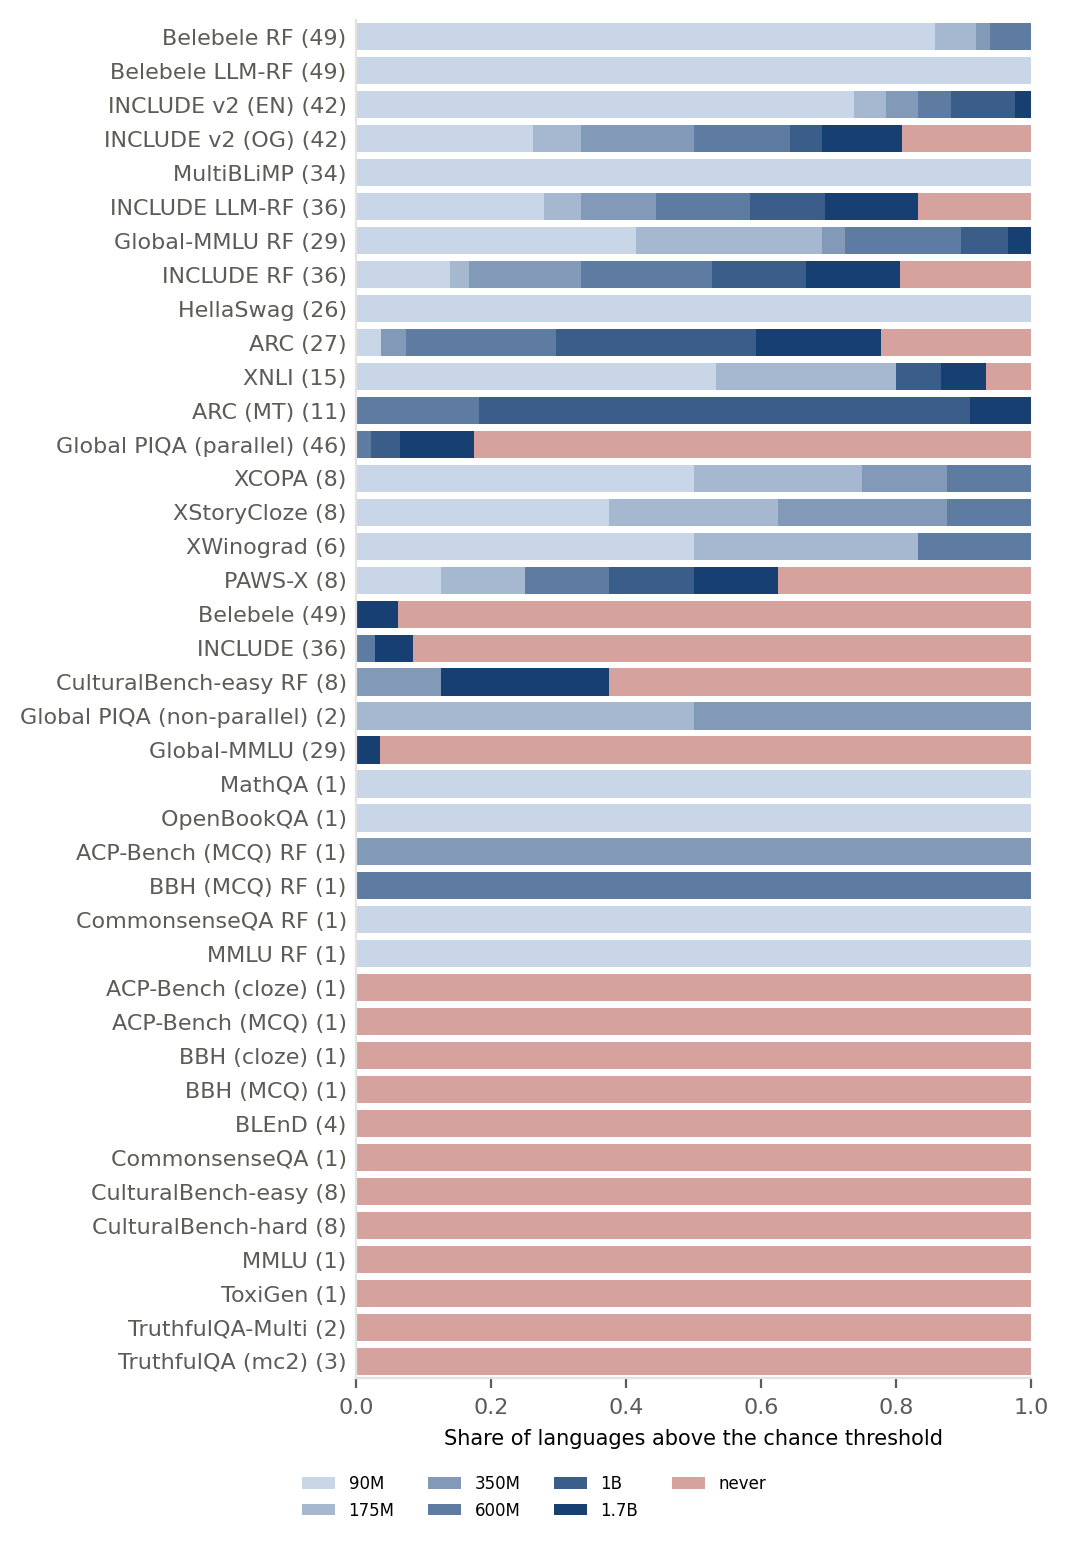
\includegraphics[width=\linewidth]{figures/app_rq00_chance_share.png}
\caption{Share of language tasks that pass the chance threshold per benchmark. The number in parentheses is the total number of language tasks available per benchmark.}
    \label{fig:app_chance_share}
\end{figure}


\begin{figure}[t]
    \centering
    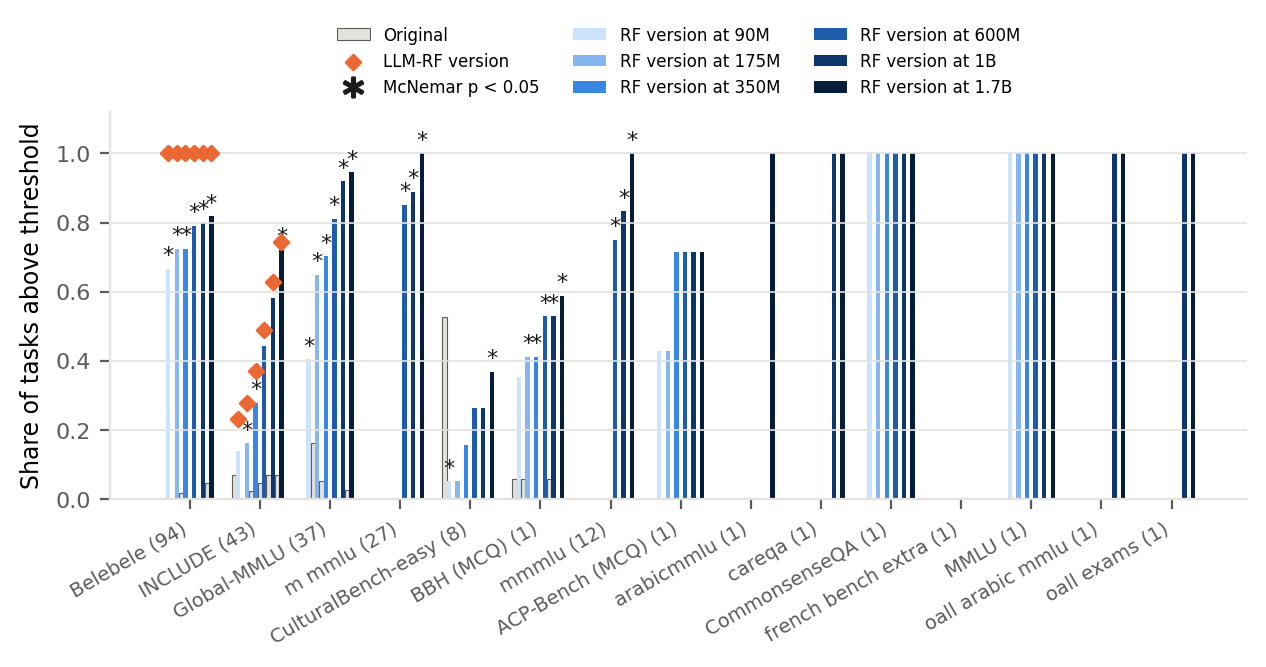
\includegraphics[width=\linewidth]{figures/app_rq00_chance_reformulation.png}
\caption{Share of language tasks that pass the chance threshold per benchmark, depending on the evaluation format.}
    \label{fig:app_chance_reformulation}
\end{figure}

\begin{figure*}[t]
    \centering
    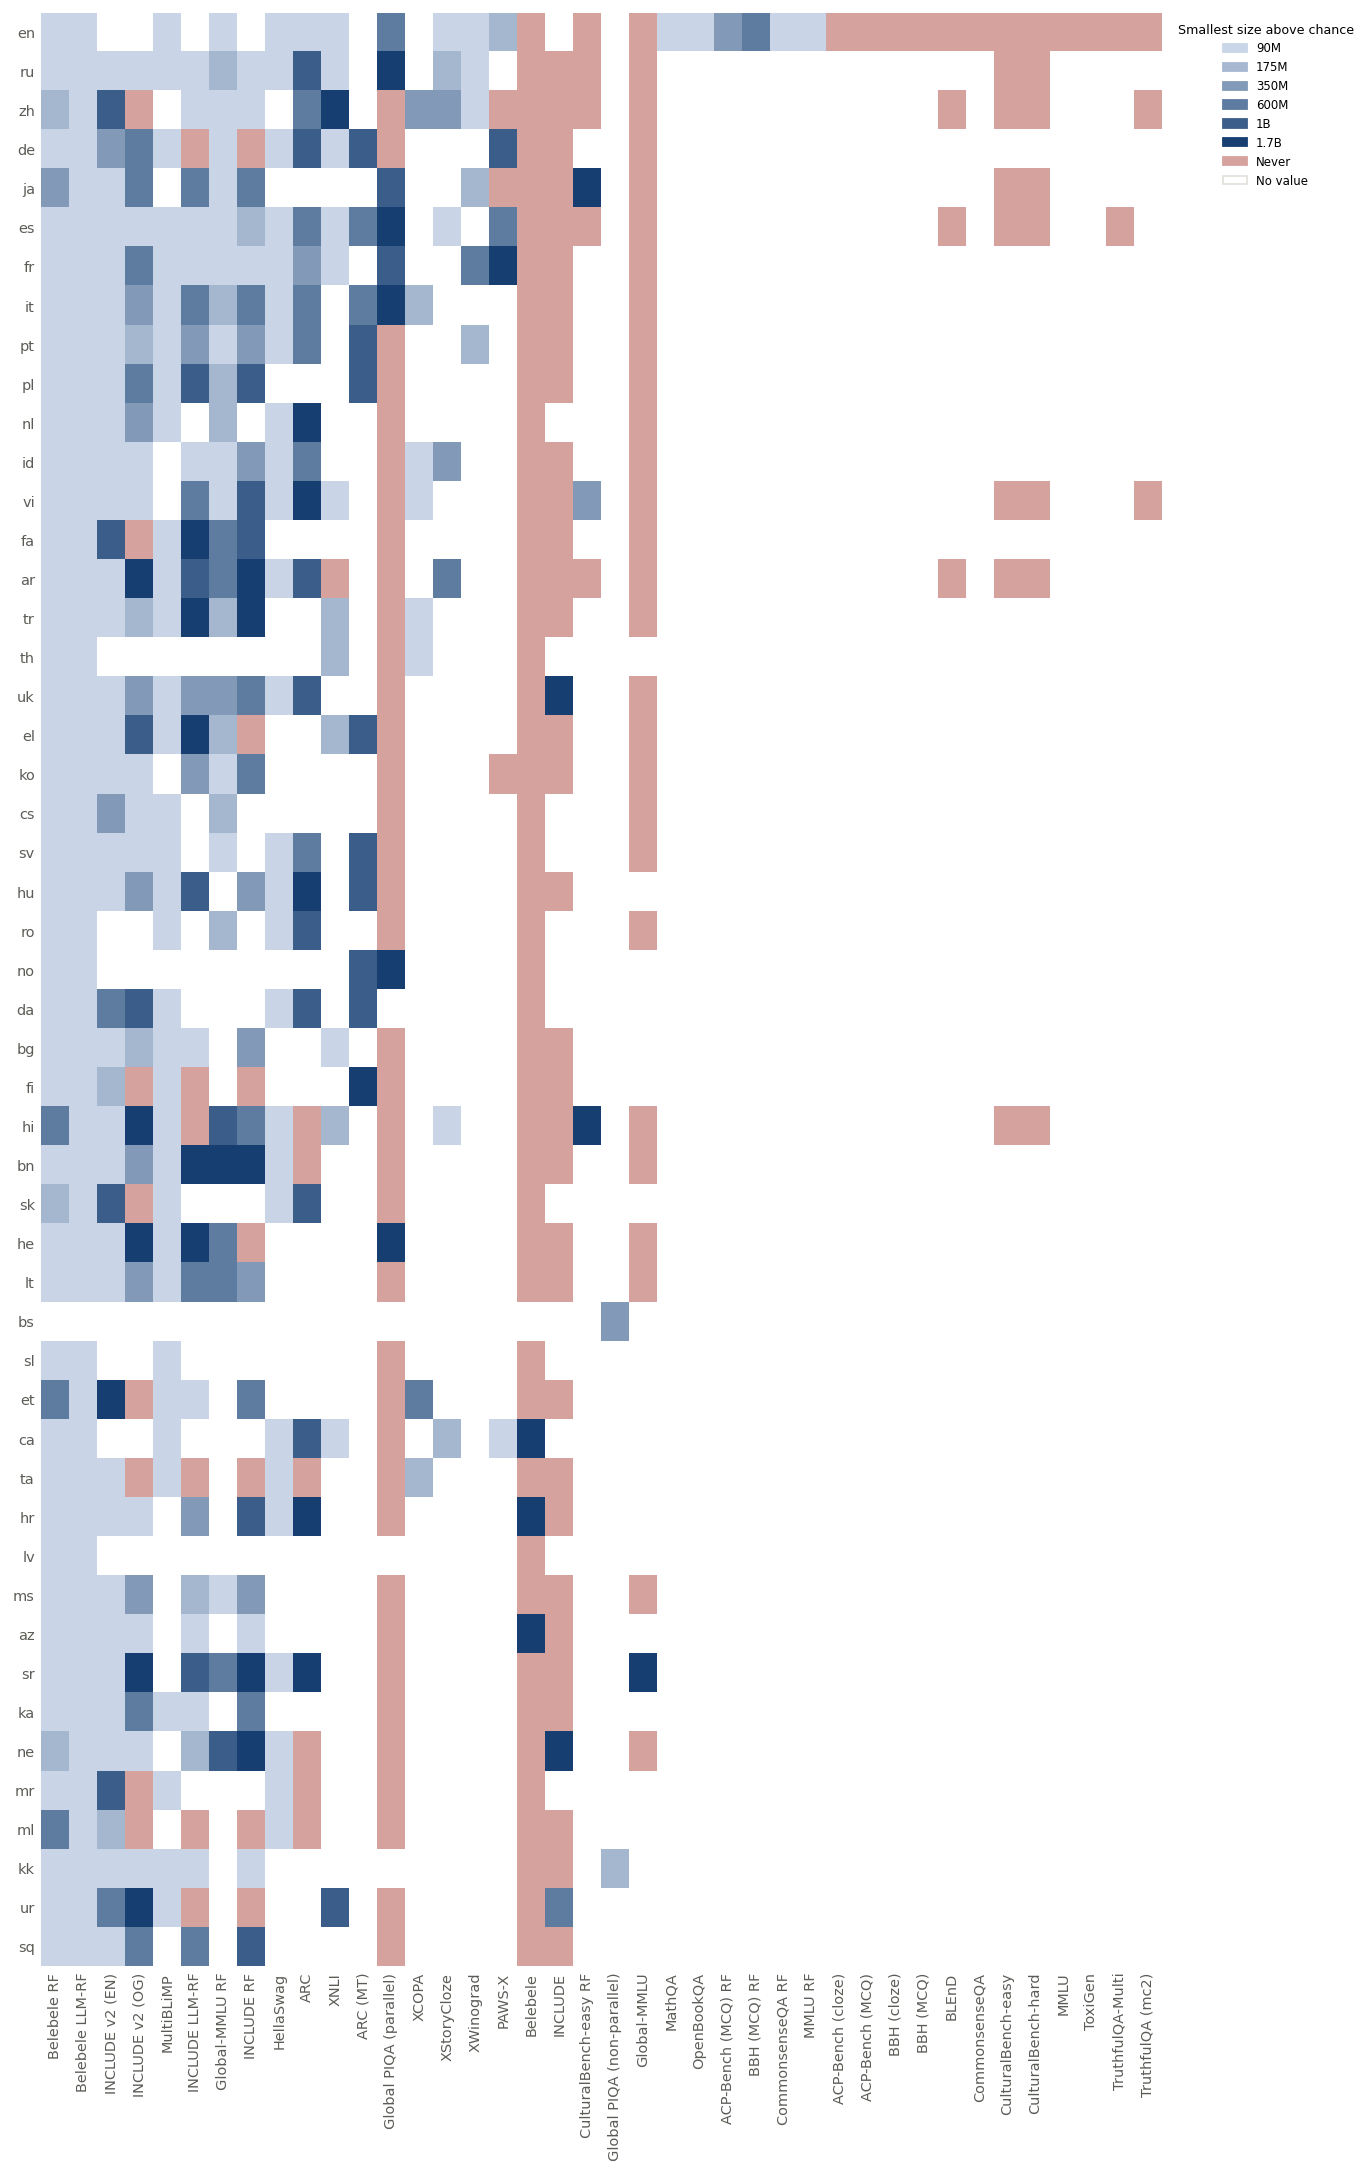
\includegraphics[width=\linewidth]{figures/app_rq00_chance_full.png}
\caption{Language tasks that pass the chance threshold per benchmark.}
    \label{fig:app_chance_full}
\end{figure*}
